\documentclass{beamer}
\mode<presentation>
{
  \usetheme{default}
  \usecolortheme{orchid} 
  \usefonttheme{professionalfonts} 
  \setbeamertemplate{navigation symbols}{}
  \setbeamertemplate{caption}[numbered]
} 
\usepackage[english]{babel}
\usepackage[utf8]{inputenc}
\usepackage[T1]{fontenc}
\usepackage{textcomp}
\usepackage{braket}
\usepackage{graphicx}
\usepackage{pgfplots}
\usepackage{booktabs}
\usepackage{adjustbox}
\usepackage{nicefrac}
\usepackage{mathtools}
\usepackage{bm}





\title[Accelerated Tempering Dynamics in HMC Simulations of Lattice Field
Theory]{Accelerated Tempering Dynamics in HMC Simulations of Lattice Field
Theory}
\author{Jack Frankland}
\institute{University of Edinburgh}
\date{\today{}}

\begin{document}

\begin{frame}
    \titlepage
\end{frame}

\section{Introduction}

    \begin{frame}{Introduction}
        \begin{itemize}
            \item<1-> What are we  doing? 
            \begin{itemize}
                \item<1-> Calculating properties of Quantum Mechanical Systems.
            \end{itemize}
            \item<2-> How are we doing it?
            \begin{itemize}
                \item<2-> Using a MCMC (Markov chain Monte Carlo) method - Hybrid Monte Carlo \cite{duane_kennedy_pendleton_roweth_1987}.
            \end{itemize}
            \item<3-> What results have we got?
            \begin{itemize}
                \item<3-> Successfully reproduced theoretical results for harmonic and anharmonic oscillators.
            \end{itemize}
            \item<4-> What is the aim?
                \begin{itemize}
                    \item<4->To improve the algorithm using \textit{tempering} dynamics - solve problem of isolated modes.
                \end{itemize}
            \item<5-> Why are we doing it?
            \begin{itemize}
                \item<5-> Can be used for calculations in lattice field theory\cite{bietenholz_2016}.
            \end{itemize}
        \end{itemize}
    \end{frame}

\section{Theory}

    \begin{frame}{The Path Integral}
        \only<1-2>
        {
           \begin{block}{Transition Amplitude}
                \only<1-2>
                {
                    \begin{equation*}
                        \label{eq:PathIntegral}
                        \braket{x_b,t_b|x_a,t_a} = \int^{x_b}_{x_a} {\cal D}{x} \exp{\left(iS_{M}\left[{x\left(t\right)}\right]\right)}
                    \end{equation*}
                Probability density of $\left(x_b,t_b\right)\rightarrow\left(x_a,t_a\right)$. \\ Integral over all paths between $\left(x_b,t_b\right)$ and $\left(x_a,t_a\right)$.
                }
            \end{block}
        }
        \only<2>
        {
            \begin{block}{Minkowski Action}
                \only<2>
                {
                    \begin{equation*}
                        \label{eq:MinkowskiAction}
                        S_{M}\left[x\left(t\right)\right] = \int^{t_b}_{t_a}dt \left[\frac{1}{2}m\left(\frac{dx}{dt}\right)^2 - V(x)\right]
                    \end{equation*}
                }
            \end{block}
        }
        \only<3>
        {  
            \begin{figure}
                \centering
                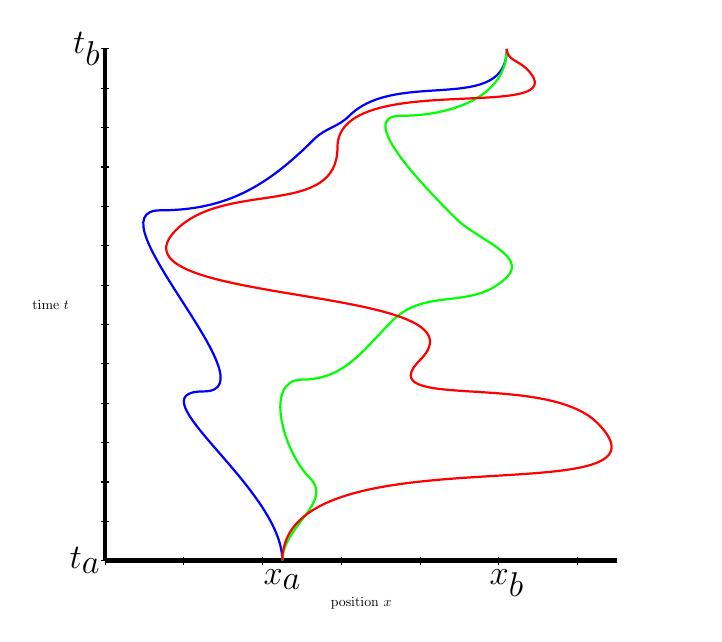
\begin{tikzpicture}[scale=0.5, every node/.style={transform shape}]
                    \draw [ultra thick] [-] (0,13) -- coordinate (y axis mid) (0,0);
                    \draw [ultra thick] [-] (0,0) -- coordinate (x axis mid) (13,0);
                    \foreach \x in {0,2,...,13}
                        \draw (\x,3pt) -- (\x,-3pt);
                    \foreach \y in {0,...,13}
                        \draw (3pt,\y) -- (-3pt,\y);
                    \node[below=0.8cm] at (x axis mid) {$\text{position}$ $x$};
                    \node[left=0.8cm] at (y axis mid) {$\text{time}$ $t$};
                    \node [left,font=\fontsize{40}{0}] at (0,0) {$t_{a}$};
                    \node [left,font=\fontsize{40}{0}] at (0,13) {$t_{b}$};
                    \node [below,font=\fontsize{40}{0}] at (4.5,-0.1) {$x_a$};
                    \node [below,font=\fontsize{40}{0}] at (10.2,-0.1) {$x_b$};
                    \draw [-,thick, blue] (4.5,0) to [out=90,in=180] (2.5,4.3)
                            to [out=0,in=180] (1.4,8.9) to [out=0,in=-135] (5.3,10.7) 
                            to [out=45,in=225] (6.2,11.3) to [out=45,in=-90] (10.2,13);
                    \draw [-,thick, green] (4.5,0) to [out=90,in=-45] (5.2,2.1)
                            to [out=135,in=180] (5.0,4.6) to [out=0,in=-135] (7.3,6.1) 
                            to [out=45,in=225] (10.2,7.2) to [out=45,in=-45] (8.9,8.7)
                            to [out=135,in=180] (7.5,11.3) to [out=0,in=-90] (10.2,13);
                    \draw [-,thick, red] (4.5,0) to [out=90,in=-45] (12.5,3.5)
                            to [out=135,in=225] (8,5.1) to [out=45,in=-135] (1.8,8.4) 
                            to [out=45,in=270] (5.9,10.5) to [out=90,in=-45] (10.7,12.5)
                            to [out=135,in=-90] (10.2,13);
                \end{tikzpicture} 
                \caption{Three possible paths from $\left(x_a,t_a\right)$ to $\left(x_b,t_b\right)$.}
            \end{figure}
        }
    \end{frame}


    \begin{frame}{Discrete Time Lattice}
        \only<1>
        {
            \begin{figure}
            \centering
            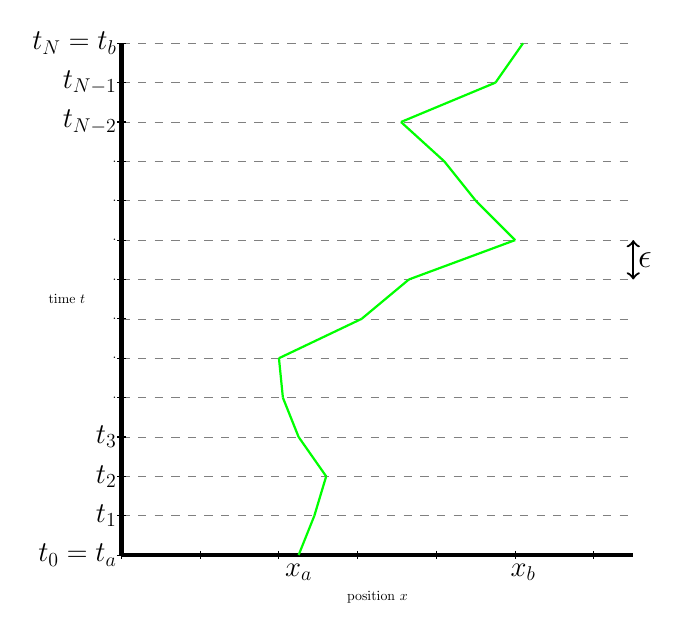
\begin{tikzpicture}[scale=0.5, every node/.style={transform shape}]
                
                \foreach \y in {0,...,13}{ \draw [help lines, dashed] (0,\y) -- (13,\y); }
                \draw [ultra thick] [-] (0,13) -- coordinate (y axis mid) (0,0);
                \draw [ultra thick] [-] (0,0) -- coordinate (x axis mid) (13,0);
                \foreach \x in {0,2,...,13}
                    \draw (\x,3pt) -- (\x,-3pt);
                \foreach \y in {0,...,13}
                    \draw (3pt,\y) -- (-3pt,\y);
                \node [left,font=\fontsize{20}{0}] at (0,0) {$t_{0}=t_{a}$};
                \node [left,font=\fontsize{20}{0}] at (0,1) {$t_{1}$};
                \node [left,font=\fontsize{20}{0}] at (0,2) {$t_{2}$};
                \node [left,font=\fontsize{20}{0}] at (0,3) {$t_{3}$};
                \node [left] at (0,4) {$.$};
                \node [left] at (0,5) {$.$};
                \node [left] at (0,6) {$.$};
                \node [left] at (0,7) {$.$};
                \node [left] at (0,8) {$.$};
                \node [left] at (0,9) {$.$};
                \node [left] at (0,10) {$.$};
                \node [left,font=\fontsize{20}{0}] at (0,11) {$t_{N-2}$};
                \node [left,font=\fontsize{20}{0}] at (0,12) {$t_{N-1}$};
                \node [left,font=\fontsize{20}{0}] at (0,13) {$t_{N}=t_{b}$};
                \node[below=0.8cm] at (x axis mid) {position $x$};
                \node[left=0.8cm] at (y axis mid) {time $t$};
                \draw [thick] [<->] (13,7) -- (13,8) ;
                \node [below=0.5cm,font=\fontsize{40}{0}] [right] at (13,8) {$\epsilon$};
                \draw [thick,green] (4.5,0) -- (4.9,1);
                \draw [thick,green] (4.9,1) -- (5.2,2);
                \draw [thick,green] (5.2,2) -- (4.5,3);
                \draw [thick,green] (4.5,3) -- (4.1,4);
                \draw [thick,green] (4.1,4) -- (4.0,5);
                \draw [thick,green] (4.0,5) -- (6.1,6);
                \draw [thick,green] (6.1,6) -- (7.3,7);
                \draw [thick,green] (7.3,7) -- (10,8);
                \draw [thick,green] (10,8) -- (9.0,9);
                \draw [thick,green] (9.0,9) -- (8.2,10);
                \draw [thick,green] (8.2,10) -- (7.1,11);
                \draw [thick,green] (7.1,11) -- (9.5,12);
                \draw [thick,green] (9.5,12) -- (10.2,13);
                \node [below,font=\fontsize{20}{0}] at (4.5,-0.1) {$x_a$};
                \node [below,font=\fontsize{20}{0}] at (10.2,-0.1) {$x_b$};
            \end{tikzpicture}
            \caption{Discretising time and a path from $\left(x_a,t_a\right)$ to $\left(x_b,t_b\right)$  onto a lattice of time spacing $\epsilon$.}
            \label{fig:TimeLattice}
        \end{figure}
        }
        %\only<3-4>
        %{
        %    
        %    \begin{block}{Discrete Notation}
        %        \only<3-4>
        %        {
        %            \begin{align}
        %            & x\left(t_j\right) = x_j \\ 
        %            \only<4>
        %            {
        %                & t_{j+1} -t_j = \epsilon
        %            }
        %            \end{align}
        %        }
        %    \end{block}
        %}
        
        \only<2->
        {
            \begin{block}{Configuration}
            \only<2->
            {
                Specific path through lattice, each lattice variable specified:
                \begin{equation*}
                    \label{eq:Configuration}
                        \bm{x} = \left(x_0,x_1,\dots,x_{N-1}\right)
                \end{equation*}
                \begin{equation*}
                    \label{eq:SiteNotation}
                        x_i=x\left(t_i\right)
                \end{equation*}
                
            }
            \end{block}
        \only<3->
        {
            \begin{block}{Wick Rotation}
                \only<3->
                {
                    Substitution for imaginary time:
                    \begin{equation*}
                    \label{eq:WickRotation}
                        \tau = it 
                    \end{equation*}
                }
                \only<4->
                {   Rotate lattice through complex plane into imaginary time of lattice spacing:
                    \begin{equation*}
                        \label{eq:WickRotationLattice}
                        a = i \epsilon
                    \end{equation*}
                }
            
            \end{block}
        }
        }
        %\only<3->
        %{
        %    
        %    \begin{block}{Discrete Minkowski Action}
        %        \only<3->
        %        {
        %        \begin{equation*}
        %            \label{eq:DiscreteMinkowskiAction}
        %            S_{M}\left(\bm{x}\right) = \sum^{N-1}_{j=0} \epsilon \left[\frac{1}{2}m\left(\frac{x_{j+1}-x_j}{\epsilon}\right)^2-V\left(x_j\right)\right]
        %        \end{equation*}
        %        }
        %    \end{block}
        %}
        
    \end{frame}
    %\begin{frame}{Discrete Time Lattice}
    %    \only<1->
    %    {
    %        \begin{block}{Integral Measure}
    %            \only<1->
    %            {
    %                \begin{equation*}
    %                    \label{eq:IntegralMeasure}
    %                    \int_{x_a}^{x_b} \mathcal{D} x \sim \int_{-\infty}^{\infty}\prod_{i=0}^{N-1}dx_i
    %                \end{equation*}
    %            }
    %        \end{block}
    %    }
    %    \only<2->
    %    {
    %       
    %       \begin{block}{Discrete Path Integral}
    %            \begin{equation*}
    %               Z \sim \int^{\infty}_{-\infty}\prod^{N-1}_{j=0}dx_{j} \exp{\left(\frac{i}{\hbar}S_{M}\left\{x_j\right\}\right)}
    %            \end{equation*}
    %        \end{block}
    %    }
    %
    %\end{frame}


    %\begin{frame}{Theory - Moving to Imaginary Time}
    %    \only<1,2,3>
    %    {
    %
    %        \begin{block}{Wick Rotation}
    %            \only<1,2,3>
    %            {
    %                \begin{equation*}
    %                \label{eq:WickRotation}
    %                    \tau = it 
    %                \end{equation*}
    %            }
    %            \only<2,3>
    %            {
    %                \begin{equation*}
    %                    \label{eq:WickRotationLattice}
    %                    a = i \epsilon
    %                \end{equation*}
    %            }
    %        \end{block}
    %    }
    %    \only<3>
    %    {
    %        \begin{block}{Discrete Euclidean Action}
    %            \only<3>
    %            {
    %
    %                \begin{align}
    %                    \label{eq:DiscreteEuclideanAction}
    %                    S_{M}\left(\bm{x}\right) & = i \sum^{N-1}_{j=0} a \left[\frac{1}{2}m\left(\frac{x_{j+1}-x_j}{a}\right)^2+V\left(x_j\right)\right] \\ 
    %                    \label{eq:EuclideanAction} & = iS_E\left(\bm{x}\right)
    %                \end{align}
    %            }
    %        \end{block}
    %    }
    %\end{frame}

    \begin{frame}{Connecting to Statistical Mechanics}
    \only<1>
        {

            \begin{block}{Discrete Euclidean Path Integral}
                \only<1>
                {  
                    \begin{equation*}
                        \label{eq:DiscreteEuclideanPathIntegral}
                        Z \sim \int^{\infty}_{-\infty}\prod^{N-1}_{j=0}dx_{j} \exp{\left(-S_E\left(\bm{x}\right)\right)}
                    \end{equation*}
                }
                Partition function of statistical mechanical system if $H\left(\bm{x}\right)=S_E\left(\bm{x}\right).$
            \end{block}
        }

        \only<2>
        {

            \begin{block}{Quantum Expectation Values}
                \only<2>
                {  
                    \begin{align*}
                        \label{eq:SpecialEXP}
                        \bra{0}\hat{A}\ket{0} & = \frac{\int^{+\infty}_{-\infty}\prod_{i=0}^{N-1}dx_i A\left(x_0,\dots,x_{N-1}\right)\exp{\left(-S_{E}\left(\bm{x}\right)\right)}}{\int^{+\infty}_{-\infty}\prod_{i=0}^{N-1}dx_i \exp{\left(-S_{E}\left(\bm{x}\right)\right)}}\\
                                             & = \langle A \rangle
                    \end{align*}
                }
            Ground state energy corresponds to statistical expectation of function $A$ on lattice.
            \end{block}
        }
    \end{frame}


\section{Numerics}

    \begin{frame}{Monte Carlo}
        \only<1-2>
        {
            \begin{block}{Expectation Value}
                Integrals cannot be computed analytically:
                \only<1-2>
                {
                \begin{equation*}
                    \label{eq:MonteCarloEstimate}
                    \langle A \rangle = \int \prod_{i=0}^{N-1}{dx_i}p\left(\bm{x}\right)A\left(\bm{x}\right)
                \end{equation*}
                }
            \end{block}
        }
        \only<2-3>
        {
            \begin{block}{Monte Carlo Estimate}
                \only<2-3>
                {
                Approximate integral as sample mean on equilibrium lattice configurations $\bm{x}_n$:
                \begin{equation*}
                    \label{eq:MonteCarloEstimate}
                    \langle A \rangle = \frac{1}{M}\sum^{M}_{n = 1} A\left(\bm{x}_{n}\right)
                \end{equation*}
                }
            \end{block}
        }
        \only<3>
        {
            \begin{block}{Boltzmann Distribution}
                \only<3>
                {
                Generate the configurations $\bm{x}_n$ according to canonical distribution:
                \begin{equation*}
                    \label{eq:BoltzmannDistribution}
                    p\left(\bm{x}\right)=\frac{1}{Z}\exp\left(-S_E\left(\bm{x}\right)\right)
                \end{equation*}
                }
            \end{block}
        }
    \end{frame}


    \begin{frame}{Hybrid Monte Carlo Algorithm - The Set Up}
        \only<1-2>
        {
            \begin{block}{Fictitious Momenta}
            \only<1-2>
            {   
                Introduce fictitious momentum variable to go with each lattice variable:
                \begin{equation*}
                    \label{eq:FictitiousMomenta}
                    \bm{p} = \left(p_0,p_1,\dots,p_{N-1}\right)
                \end{equation*}
            }
            \end{block}
        }
        \only<2>
        {
            \begin{block}{HMC Hamiltonian}
                \only<2>
                {
                Hamiltonian for the joint canonical but separable distribution of $\left(\bm{x},\bm{p}\right)$:
                \begin{equation*}
                    \label{eq:HMCHamiltonian}
                    H_{HMC}\left(\bm{x},\bm{p}\right) \coloneqq \sum_{i=0}^{N-1} \frac{ p_{i}^{2} } {2} + S_{E}\left(\bm{x}\right)
                \end{equation*}
                }
            \end{block}
        }
    \end{frame}
    \begin{frame}{The Hybrid Monte Carlo Algorithm}
        \only<1->
        {
            \begin{block}{HMC Algorithm}
                \begin{enumerate} 
                    \setcounter{enumi}{-1}

                    \item<1-> Provide initial configuration $\bm{x}$.

                    \item<2-> Generate $\bm{p}$ from $\mathcal{N}\left(\bm{0},\mathbb{I}\right)$.

                    \item<3-> Evolve $\left(\bm{x}, \bm{p}\right)$ using Hamilton's equations (leapfrog method) to a final state $\left(\bm{x}', \bm{p}'\right)$.

                    \item<4-> Accept configuration $\bm{x}$ with probability $ \min{\left[1,\exp{\left(-H_{HMC}\left(\bm{x}',\bm{p}'\right)+H_{HMC}\left(\bm{x},\bm{p}\right)\right)}\right]}$ (Metropolis update).

                    \item<5-> Return to step $1$.
                \end{enumerate}
            \end{block}
        } 
    \end{frame}

\section{Results}
    \begin{frame}{Harmonic Oscillator}
        \only<1-2>
        {
        \begin{block}{The potential}
            \begin{equation*}
            V\left(x\right) = \frac{\mu^2}{2}x^2
            \end{equation*}
        \end{block}
        }
        \only<2>
        {
        \begin{block}{The HMC Hamiltonian}
            \begin{equation*}
            H_{HMC}\left(\bm{x},\bm{p}\right) = \sum_{i=0}^{N-1} \frac{p_i^2}{2} + \sum_{i=0}^{N-1} a \left[\frac{1}{2}m\left(\frac{x_{i+1}-x_{i}}{a}\right)^2 + \frac{1}{2}\mu^2x_i^2\right]
            \end{equation*}
        \end{block}
        }
    \end{frame}
    
    \begin{frame}{Harmonic Oscillator Typical Configuration}
        \only<1>
        {
            \begin{figure}
                    \centering
                        \begin{tikzpicture}[scale=1]
                            \begin{axis}[
                                xlabel= {$x$},
                                ylabel style ={rotate=0},
                                ylabel= {Lattice Site},
                                enlargelimits=true,
                                        ]
                                \addplot[color=black,mark=x,skip coords between index={100}{1000}]
                                table[x index=1, y index=0]{../Report/DataForReport/HarmonicTypicalTrajectory.dat};
                            \end{axis}
                        \end{tikzpicture}
                        \label{fig:TypicalHarmonicPath}
                        \caption{Typical equilibrium configuration on $100$ site lattice at spacing $a=1$ with harmonic potential $\mu=1$.}
                \end{figure}
        }
    \end{frame}

    \begin{frame}{Harmonic Oscillator Expectation Values}
        \only<1->
        {
            \begin{figure}
                    \centering
                    \begin{tikzpicture}[scale=1]
                        \begin{axis}[
                            legend style={font=\tiny},
                            xlabel= {$a$},
                            ylabel style ={rotate=-90},
                            ylabel= {$\braket{x^2}$},
                            enlargelimits=true,
                                    ]
                            \addplot[only marks, 
                                   mark=x,color=black]
                                plot [error bars/.cd, 
                                    y dir = both, 
                                    y explicit]
                                table[x index=0, 
                                    y index=1, 
                                    y error index=2]{../Report/DataForReport/LatticeSpacingvsExpectationXSquared.dat};
                            \addlegendentry{Measured Values}
                            \addplot[domain=0.1:1,
                                samples=100,
                                color=blue,
                                    ]
                                {(1/2)*(1/sqrt(1+0.25*x*x)) * ((1+(1+0.5*x*x-x*sqrt(1+0.25*x*x))^(100))/((1-(1+0.5*x*x-x*sqrt(1+0.25*x*x))^(100))))};
                         \addlegendentry{Discrete Theory}      
                        \end{axis}
                    \end{tikzpicture}
                    \label{fig:MeanXSquaredPlot}
                    \caption{Mean position squared for a range of finite lattice spacings on a $100$ site lattice with harmonic potential $\mu=1$.}
                \end{figure}
        }
    \end{frame}

    \begin{frame}{Harmonic Oscillator Ground State Probability Density}
        \only<1>
        {
        \begin{figure}
                    \centering
                    \begin{tikzpicture}[scale=1]
                        \begin{axis}[
                            legend style={font=\fontsize{4}{5}\selectfont},
                            xlabel= {$x$},
                            ylabel style ={rotate=-90},
                            ylabel= {$\left|\psi{\left(x \right)}\right|^2$},
                            enlargelimits=true,
                                    ]
                            \addplot[only marks, 
                                mark=x,color=black]
                                plot[error bars/.cd, 
                                    y dir = both, 
                                    y explicit]
                                table[x index=0, 
                                y index=1, 
                                y error index=2]{../Report/DataForReport/HarmonicWaveFunction.dat};
                            \addlegendentry{Measured Values}
                            \addplot[domain=-4:4,
                                samples=100,
                                color=blue,
                                    ]
                                {sqrt(sqrt(5)/(2*pi))*e^(-0.5*sqrt(5)*x*x)};
                            \addlegendentry{Discrete Theory}
                            \addplot[domain=-4:4,
                                samples=100,
                                color=red,
                                    ]
                                {1/sqrt(pi)*e^-x*x};
                            \addlegendentry{Continuum Theory}
                        \end{axis}
                    \end{tikzpicture}
                    \label{fig:HarmonicWaveFunction}
                    \caption{Ground state probability density function for $100$ site lattice at spacing $a=1$ for harmonic potential $\mu=1$.}
                \end{figure}
            
        }

        %\only<2>
        %{
        %    \begin{block}{Discrete Wave Function\footfullcite{creutz_freedman_1981}}
        %        \only<2>
        %        {
        %            \begin{equation*}
        %                \label{eq:DiscreteWaveFunction}
        %                \psi_{disc.}{\left(x\right)} = \left(\frac{\omega}{\pi}\right)^\frac{1}{4}\exp{\left(-\frac{1}{2}\omega x^2\right)}
        %            \end{equation*}
        %        }
        %        \only<2>
        %        {
        %            \begin{equation*}
        %            \omega^2 = \mu^2\left(1+\frac{a^2 \mu^2}{4}\right)
        %            \end{equation*}
        %        }
                %\only<6>{
                %\begin{equation*}
                %\left| \psi_{disc.}{\left(x\right)} \right|^2 = \sqrt{\frac{\sqrt{5}}{2\pi}}\exp{\left(-\frac{1}{2}\sqrt{5}{\omega} x^2\right)}
                %\end{equation*}}
        %    \end{block}
        %}
        %\only<5>{\begin{block}{Continuous Wave Function}
        %\only<5>{
        %\begin{equation*}
        %\label{eq:ContinuousWaveFunction}
        %\psi_{cont.}{\left(x\right)} = \left(\frac{\mu}{\pi}\right)^\frac{1}{4}\exp{\left(-\frac{1}{2}\mu x^2\right)}
        %\end{equation*}}
        %\only<10>{
        %\begin{equation*}
        %\left| \psi_{cont.}{\left(x\right)} \right|^2 = \frac{1}{\sqrt{2\pi}}\exp{\left(-x^2\right)}
        %\end{equation*}}
        %\end{block}}
    \end{frame}
    %
    %\begin{frame}{Results - Harmonic Oscillator Lattice spacing vs. $\braket{x^2}$}
    %
    %    \only<3-4>{
    %        \begin{block}{$\braket{x^2}$ on a lattice \footfullcite{creutz_freedman_1981}}
    %            \only<3-4>{
    %                \begin{equation*}
    %                    \braket{x^2} = \frac{1}{2\left(1+\frac{1}{4}a^2\right)^{\frac{1}{2}}}\left(\frac{1+R^n}{1-R^n}\right)
    %                \end{equation*}
    %            }
    %    
    %            \only<4>{
    %                \begin{equation*}
    %                    R = 1 + \frac{a^2\mu^2}{2}-a\mu\left(1+\frac{a^2\mu^2}{4}\right)^{\frac{1}{2}}
    %                \end{equation*}}
    %        \end{block}
    %    }
    %
    %    \only<2,5->{\begin{figure}
    %    \centering
    %        \begin{tikzpicture}
    %            \begin{axis}[
    %                legend style={font=\tiny},
    %                xlabel= {$a$},
    %                ylabel style ={rotate=-90},
    %                ylabel= {$\braket{x^2}$},
    %                enlargelimits=true,
    %                ]
    %                \only<2,5->{\addplot[only marks, 
    %                                   mark=x,color=black]
    %                            plot [error bars/.cd, 
    %                                    y dir = both, 
    %                                    y explicit]
    %                            table[x index=0, 
    %                                  y index=1, 
    %                                  y error index=2]{DataForPresentation/LatticeSpacingvsExpectationXSquared.dat};
    %                    \addlegendentry{Measured Values}}
    %                \only<5->{\addplot[domain=0:1,
    %                         samples=100,
    %                         color=blue,
    %                         ]
    %                         {(1/2)*(1/sqrt(1+0.25*x*x)) * ((1+(1+0.5*x*x-x*sqrt(1+0.25*x*x))^(1000))/((1-(1+0.5*x*x-x*sqrt(1+0.25*x*x))^(1000))))};
    %                         \addlegendentry{Discrete Theory}}
    %                         
    %
    %            \end{axis}
    %        \end{tikzpicture}
    %        \note[item]{Relationship between lattice spacing and expectation of position squared for the harmonic oscillator with $\mu^2 = 1, m = 1, a = 1, L = 1000, d = 0.1, N = 10, \text{configurations} = 100000, \text{burn period} = 1000$.}
    %    \end{figure}}   
    %\end{frame}

    %\begin{frame}{Results - Anharmonic Oscillator Potential}
    %    \only<2->{\begin{figure}
    %    \centering
    %        \begin{tikzpicture}
    %            \begin{axis}[
    %                legend style={font=\tiny},
    %                xlabel= {$x$},
    %                ylabel= {$V(x)$},
    %                ylabel style ={rotate=-90},
    %                enlargelimits=true,
    %                ]
    %                \addplot[domain=-4:4, samples=100, color=black,]{x^4-8*x^2+16};
    %                \addlegendentry{$V(x)=\lambda\left(x^2-f^2\right)^2$}
    %
    %            \end{axis}
    %        \end{tikzpicture}
    %        \note[item]{Anharmonic Oscillator Potential with $\lambda = 1, f^2 = 4$.}
    %    \end{figure}}
    %\end{frame}
    \begin{frame}{Anharmonic Oscillator}
    \only<3>
    {
       \begin{figure}
        \centering
            \begin{tikzpicture}
                \begin{axis}[
                    legend style={at={(0.5,1.01)},anchor=north,font=\tiny},
                    xlabel= {$x$},
                    ylabel style ={rotate=-90},
                 ylabel= {$V(x)$},
                   enlargelimits=true,
                   ytick={0},
                   xtick={-2,0,2},
                   xticklabels={-$f$,$0$,$f$},
                   yticklabels={$0$}
                   ]
                   \addplot[domain=-3:3, samples=100, color=black,]{(x*x-4)*(x*x-4)};
                   \addlegendentry{$V(x)=\lambda\left(x^2-f^2\right)^2$}
                   \draw [gray,dashed] (axis cs: -2,-1) -- (axis cs: -2,30.1);
                   \draw [gray,dashed] (axis cs: 2,-1) -- (axis cs: 2,30.1);
    
               \end{axis}
           \end{tikzpicture}
           \caption{Anharmonic potential parameterisation, wells coincide with minima at $\pm f$ forming symmetric double wells.}
        \end{figure}
    }
        \only<1-2>
        {
        \begin{block}{The potential}
            \begin{equation*}
            V\left(x\right) = \lambda\left(x^2-f^2\right)^2
            \end{equation*}
        \end{block}
        }
        \only<2>
        {
        \begin{block}{The HMC Hamiltonian}
            \begin{equation*}
            H_{HMC}\left(\bm{x},\bm{p}\right) = \sum_{i=0}^{N-1} \frac{p_i^2}{2} + \sum_{i=0}^{N-1} a \left[\frac{1}{2}m\left(\frac{x_{i+1}-x_{i}}{a}\right)^2 + \lambda\left(x_i^2-f^2\right)^2\right]
            \end{equation*}
        \end{block}
        }


    \end{frame}

    \begin{frame}{Anharmonic Oscillator Typical Configuration}
        \only<1>
        {
            \begin{figure}
                    \centering
                    \begin{tikzpicture}[scale=1]
                        \begin{axis}[
                            xlabel= {$x$},
                            ylabel style ={rotate=0},
                            ylabel= {Lattice Site},
                            enlargelimits=true,
                                    ]
                            \addplot[color=black,mark=x,skip coords between index={100}{1000}]
                            table[x index=1, y index=0]{../Report/DataForReport/AnharmonicTypicalTrajectory.dat};
                            
                            \draw [gray,dashed] (axis cs: -2,-10) -- (axis cs: -2,110);
                            \draw [gray,dashed] (axis cs: 2,-10) -- (axis cs:2,110);
                        \end{axis}
                    \end{tikzpicture}
                    \label{fig:TypicalAnharmonicTrajectory}
                    \caption{Typical equilibrium configuration on $100$ site lattice at spacing $a=1$ with anharmonic potential $\lambda=1, f=1$.}
                \end{figure}
        }
    \end{frame}

    \begin{frame}{Anharmonic Oscillator Expectation Values}
        \only<1->
        {
            \begin{figure}
                    \centering
                    \begin{tikzpicture}[scale=1]
                        \begin{axis}[
                            legend style={font=\tiny},
                            xlabel= {$f^2$},
                            ylabel style ={rotate=0},
                            ylabel= {Energy},
                            enlargelimits=true,
                                    ]
                            \addplot[color=red,mark=x,]
                            table[x index=0, y index=1]{../Report/DataForReport/ReferenceAnharmonicGroundstateEnergies.dat};
                            \addlegendentry{Reference $E_0$ \cite{blankenbecler_degrand_sugar_1980}}

                            \addplot[color=red,mark=o,]
                            table[x index=0, y index=1]{../Report/DataForReport/ReferenceAnharmonicFirstExcitedStateEnergies.dat};
                            \addlegendentry{Reference $E_1$ \cite{blankenbecler_degrand_sugar_1980}}

                            \addplot[color=blue,mark=x,]
                            plot [error bars/.cd, y dir = both, y explicit]
                            table[x index=0, y index=1, y error index=2]{../Report/DataForReport/MeasuredAnharmonicGroundstateEnergiesa1.dat};
                            \addlegendentry{Measured $E_0$}

                            \addplot[color=blue,mark=o,]
                            plot [error bars/.cd, y dir = both, y explicit]
                            table[x index=0, y index=1, y error index=2]{../Report/DataForReport/MeasuredFirstExcitedStateEnergiesa1.dat};
                            \addlegendentry{Measured $E_1$}            
                        \end{axis}
                    \end{tikzpicture}
                    \label{fig:AnharmonicEnergies}
                    \caption{Ground and first excited state energy eigenvalues on $1000$ site lattice at spacing $a=0.1$ with anharmonic potential $\lambda=1$ for a range of $f$ values.}
                \end{figure}
        }
    \end{frame}

    \begin{frame}{Anharmonic Oscillator Ground State Density Function}
        \only<1>
        {
            \begin{figure}
                    \centering
                    \begin{tikzpicture}[scale=1]
                        \begin{axis}[
                            legend style={at={(0.5,1.01)},anchor=north,font=\tiny},
                            xlabel= {$x$},
                            ylabel style ={rotate=-90},
                            ylabel= {$\left|\psi{\left(x \right)}\right|^2$},
                            enlargelimits=true,
                            ymax=0.6
                                    ]
                        \addplot[color=black,mark=x,]
                            plot [error bars/.cd, y dir = both, y explicit]
                            table[x index=0, y index=1, y error index=2]{../Report/DataForReport/AnharmonicWaveFunction.dat};
                            \draw [gray,dashed] (axis cs: -1,-0.1) -- (axis cs: -1,1.1);
                            \draw [gray,dashed] (axis cs: 1,-0.1) -- (axis cs: 1,1.1);
                            \node [draw,below=0.5cm] [right] at (axis cs: -4,0.6) {$\langle x \rangle = 0.000760909 \pm 0.000930068$};
                        \end{axis}
                    \end{tikzpicture}
                    \label{fig:AnharmonicWaveFunction}
                    \caption{Ground state probability density function on $100$ site lattice of spacing $a=1$ with anharmonic potential $\lambda=1,f=1$.}
                \end{figure}
        }
    \end{frame}

    \begin{frame}{Isolated Modes \textcolor{black}{$\lambda=1,f=1$}}

        \only<1>
        {
           \begin{figure}
                \begin{tikzpicture}
                    \begin{axis}[
                        legend style={font=\tiny},
                        xlabel= {$x$},
                        ylabel style ={rotate=0},
                        ylabel= {Lattice Site},
                        enlargelimits=true,
                        legend style={at={(0.5,1.01)},anchor=west}
                                ]
                        \addplot[color=green,mark=none]
                        table[x index=1, y index=0]{../Report/DataForReport/f1initialconfig.dat};
                        \addlegendentry{Initial Equilibrium Configuration}
                        \addplot[color=red,mark=none]
                        table[x index=1, y index=0]{../Report/DataForReport/f1finalconfig.dat};
                        \addlegendentry{Final Equilibrium Configuration}
                        \draw [gray,dashed] (axis cs: -1,-10) -- (axis cs: -1,120);
                        \draw [gray,dashed] (axis cs: 1,-10) -- (axis cs:1,120);
                    \end{axis}
                \end{tikzpicture}
                \caption{Initial and final equilibrium configurations after $100000$ iterations on $100$ site lattice at spacing $a=1$.}
                \label{fig:initialfinalf2}
            \end{figure}
        }
    \end{frame}
    \begin{frame}{Isolated Modes \textcolor{black}{$\lambda=1,f=\sqrt{3}$}}
            \begin{figure}
                \begin{tikzpicture}
                    \begin{axis}[
                        legend style={font=\tiny},
                        xlabel= {$x$},
                        ylabel style ={rotate=0},
                        ylabel= {Lattice Site},
                        enlargelimits=true,
                        legend style={at={(0.5,1.01)},anchor=west}
                                ]
                        \addplot[color=green,mark=none]
                        table[x index=1, y index=0]{../Report/DataForReport/f3initialconfig.dat};
                        \addlegendentry{Initial Equilibrium Configuration}
                        \addplot[color=red,mark=none]
                        table[x index=1, y index=0]{../Report/DataForReport/f3finalconfig.dat};
                        \addlegendentry{Final Equilibrium Configuration}
                        \draw [gray,dashed] (axis cs: -1.732,-10) -- (axis cs: -1.732,120);
                        \draw [gray,dashed] (axis cs: 1.732,-10) -- (axis cs:1.732,120);
                    \end{axis}
                \end{tikzpicture}
                \caption{Initial and final equilibrium configurations after $100000$ iterations on $100$ site lattice at spacing $a=1$.}
                \label{fig:initialfinalf2}
            \end{figure}
    \end{frame}
    \begin{frame}{Isolated Modes \textcolor{black}{$\lambda=1,f=\sqrt{3}$}}
        \begin{figure}
                    \centering
                    \begin{tikzpicture}[scale=1]
                        \begin{axis}[
                            xlabel= {$x$},
                            ylabel style={rotate=-90},
                            ylabel= {$\left|\psi{\left(x \right)}\right|^2$},
                            enlargelimits=true,
                                    ]
                            \addplot[color=black,mark=x,]
                            plot [error bars/.cd, y dir = both, y explicit]
                            table[x index=0, y index=1, y error index=2]{../Report/DataForReport/f3isolatedmodewavefunction.dat};
                            \draw [gray,dashed] (axis cs: -1.732,-10) -- (axis cs: -1.732,120);
                            \draw [gray,dashed] (axis cs: 1.732,-10) -- (axis cs:1.732,120);
                            \node [draw,below=0.5cm] [align=right] at (axis cs: -2,1.5) {$\langle x \rangle = 0.618997\pm $ \\ $
                            0.00135925$};

                        \end{axis}
                    \end{tikzpicture}
                    \caption{Asymmetric density function and non zero mean position.}
    
        \end{figure}
        
    \end{frame}
    \begin{frame}{Isolated Modes \textcolor{black}{$\lambda=1,f=2$}}
            \begin{figure}
                \begin{tikzpicture}
                    \begin{axis}[
                        legend style={font=\tiny},
                        xlabel= {$x$},
                        ylabel style ={rotate=0},
                        ylabel= {Lattice Site},
                        enlargelimits=true,
                        legend style={at={(0.5,1.01)},anchor=west}
                                ]
                        \addplot[color=green,mark=none]
                        table[x index=1, y index=0]{../Report/DataForReport/f4initialconfig.dat};
                        \addlegendentry{Initial Equilibrium Configuration}
                        \addplot[color=red,mark=none]
                        table[x index=1, y index=0]{../Report/DataForReport/f4finalconfig.dat};
                        \addlegendentry{Final Equilibrium Configuration}
                        \draw [gray,dashed] (axis cs: -2,-10) -- (axis cs: -2,120);
                        \draw [gray,dashed] (axis cs: 2,-10) -- (axis cs: 2,120);
                    \end{axis}
                \end{tikzpicture}
                \caption{Initial and final equilibrium configurations after $100000$ iterations on $100$ site lattice at spacing $a=1$.}
                \label{fig:initialfinalf4}
            \end{figure}
    \end{frame}
    \begin{frame}{Isolated Modes \textcolor{black}{$\lambda=1,f=2$}}
        \begin{figure}
                    \centering
                    \begin{tikzpicture}[scale=1]
                        \begin{axis}[
                            xlabel= {$x$},
                            ylabel style={rotate=-90},
                            ylabel= {$\left|\psi{\left(x \right)}\right|^2$},
                            enlargelimits=true,
                            ymax=1.3
                                    ]
                            \addplot[color=black,mark=x,]
                            plot [error bars/.cd, y dir = both, y explicit]
                            table[x index=0, y index=1, y error index=2]{../Report/DataForReport/f4isolatedmodewavefunction.dat};
                            \draw [gray,dashed] (axis cs: -2,-10) -- (axis cs: -2,120);
                            \draw [gray,dashed] (axis cs: 2,-10) -- (axis cs: 2,120);
                            \node [draw,align=right] at (axis cs: 1,1.2) {$\langle x \rangle = −0.102023\pm$ \\ $0.000516574$};

                        \end{axis}
                    \end{tikzpicture}
                    \caption{Asymmetric density function and non zero mean position.}
        \end{figure}
    \end{frame}

    \begin{frame}{Tempering}
    \begin{itemize}
            \item<1-> What is tempering? 
            \begin{itemize}
                \item<1-> Method to sample from more diffuse probability distribution.
            \end{itemize}
            \item<2-> How is it incorporated into HMC?
            \begin{itemize}
                \item<2-> Multiply (divide) momentum variables during the numerical integration of Hamilton's equations by a tempering parameter $\alpha$ in first (second) half of the trajectory \cite{neal_2011}.
            \end{itemize}
            \item<3-> What results would we expect?
            \begin{itemize}
                \item<3-> Better estimates on expectation values and less correlation between configurations.
            \end{itemize}
        \end{itemize}
    \end{frame}
    \begin{frame}{Leapfrog Integration}
    \only<1-2>
    {
    \begin{block}{Hamiltonian}
        Form of Hamiltonian for our simulation:
        \begin{equation*}
            \label{eq:HamiltonianUPlusK}
            H\left(\bm{q},\bm{p}\right) = U\left(\bm{q}\right) + K\left(\bm{p}\right)
        \end{equation*}
    \end{block}
    }
    \only<2>
    {
    \begin{block}{Leapfrog Equations}
        Half step in momentum then full step in position then half step in position to go from $t$ to $t+\epsilon$: 
        \begin{align*}
                p_i\left(t+\epsilon/2\right) &  = p_i\left(t\right) - \epsilon/2\frac{\partial U}{\partial q_i}\left(\bm{q}\left(t\right)\right) \\
                q_i\left(t+\epsilon\right) &  = q_i\left(t\right) + \epsilon\frac{\partial K}{\partial p_i}\left(\bm{p}\left(t+\epsilon/2\right)\right) \\
                p_i\left(t+\epsilon\right) &  = p_i\left(t+\epsilon/2\right) - \epsilon/2\frac{\partial U}{\partial q_i}\left(\bm{q}\left(t+\epsilon\right)\right)
            \end{align*}
    \end{block}
    }
    \only<3>
    {
        \begin{block}{Tempered Leapfrog Equations First Half Trajectory}
            Multiply momentum variables by $\sqrt{\alpha}$ before first half step in momentum and after second half step during second half of trajectory:
            \begin{align*}
                 p_i\left(t+\epsilon/2\right) & = \sqrt{\alpha}p_i\left(t\right) - \epsilon/2\frac{\partial U}{\partial q_i}\left(\bm{q}\left(t\right)\right) \\
                \label{eq:TLeapFrogEq2}q_i\left(t+\epsilon\right) & = q_i\left(t\right) + \epsilon\frac{\partial K}{\partial p_i}\left(\bm{p}\left(t+\epsilon/2\right)\right) \\
                \label{eq:TLeapFrogEq3}p_i\left(t+\epsilon\right) & = \sqrt{\alpha}\left(p_i\left(t+\epsilon/2\right) - \epsilon/2\frac{\partial U}{\partial q_i}\left(\bm{q}\left(t+\epsilon\right)\right)\right)
            \end{align*}
        \end{block}
    }
    \only<4>
    {
        \begin{block}{Tempered Leapfrog Equations Second Half Trajectory}
        Divide momentum variables by $\sqrt{\alpha}$ before first half step in momentum and after second half step during first half of trajectory:
            \begin{align*}
                p_i\left(t+\epsilon/2\right) & = \frac{1}{\sqrt{\alpha}}p_i\left(t\right) - \epsilon/2\frac{\partial U}{\partial q_i}\left(\bm{q}\left(t\right)\right) \\
                q_i\left(t+\epsilon\right) & = q_i\left(t\right) + \epsilon\frac{\partial K}{\partial p_i}\left(\bm{p}\left(t+\epsilon/2\right)\right) \\
                p_i\left(t+\epsilon\right) & = \frac{1}{\sqrt{\alpha}}\left(p_i\left(t+\epsilon/2\right) - \epsilon/2\frac{\partial U}{\partial q_i}\left(\bm{q}\left(t+\epsilon\right)\right)\right)
            \end{align*}
        \end{block}
    }
\end{frame}

    \begin{frame}{Molecular Dynamics Hamiltonian Evolution \large\textcolor{black}{$\alpha=1.001$}}
    \begin{figure}
    \centering
    \begin{tikzpicture}[scale=1]
                            \begin{axis}[
                                xlabel= {Leapfrog Steps},
                                ylabel style ={rotate=-90},
                                ylabel= {$H_{HMC}$},
                                enlargelimits=true,
                                        ]
                                \addplot[color=black,mark=none,]
                                table[x index=0, y index=1]{../Report/DataForReport/1001HamiltonianEvolution.dat};
                                \draw [gray,dashed] (axis cs: 0,197.369) -- (axis cs: 200,197.369);
                                \draw [gray,dashed] (axis cs: 0,197.298) -- (axis cs: 200,197.298);
                                \node [draw,align=right] at (axis cs: 100,200) {$\Delta H_{HMC} = -0.071$};

                            \end{axis}
                        \end{tikzpicture}
                        \caption{Evolution of HMC Hamiltonian along tempered leapfrog trajectory for $100$ site lattice at spacing $a=1$ with anharmonic potential $\lambda=1,f=2$.}
                        
  \end{figure}%% 
  
  \end{frame}
  \begin{frame}{Molecular Dynamics Configuration Evolution \large\textcolor{black}{$\alpha=1.001$}}
  \begin{figure}
    \centering
    \begin{tikzpicture}[scale=1]
                            \begin{axis}[
                                xlabel= {$x$},
                                ylabel style ={rotate=0},
                                ylabel= {Lattice Site},
                                enlargelimits=true,
                                legend style={at={(0.5,1.01)},anchor=west,font=\tiny}
                                        ]
                                \addplot[color=green,mark=none,]
                                table[x index=1, y index=0]{../Report/DataForReport/1001ConfigurationEvolution1.dat};
                                \addlegendentry{Initial Configuration}
                                \addplot[color=red,mark=none,]
                                table[x index=1, y index=0]{../Report/DataForReport/1001ConfigurationEvolution2.dat};
                                \addlegendentry{Configuration at 100 leapfrog steps}
                                \addplot[color=blue,mark=none,]
                                table[x index=1, y index=0]{../Report/DataForReport/1001ConfigurationEvolution3.dat};
                                \addlegendentry{Proposal Configuration}
                                \draw [gray,dashed] (axis cs: -2,-10) -- (axis cs: -2,120);
                                \draw [gray,dashed] (axis cs: 2,-10) -- (axis cs: 2,120);



                            \end{axis}
                        \end{tikzpicture}
                        \caption{Evolution of the equilibrium configuration along the tempered leapfrog trajectory.}
                        
  \end{figure} 

\end{frame}
\begin{frame}{Molecular Dynamics Hamiltonian Evolution \large\textcolor{black}{$\alpha=1.01$}}
  \begin{figure}
    \centering
    \begin{tikzpicture}[scale=1]
                            \begin{axis}[
                                xlabel= {Leapfrog Steps},
                                ylabel style ={rotate=-90},
                                ylabel= {$H_{HMC}$},
                                enlargelimits=true,
                                        ]
                                \addplot[color=black,mark=none,]
                                table[x index=0, y index=1]{../Report/DataForReport/101HamiltonianEvolution.dat};
                                \draw [gray,dashed] (axis cs: 0,197.369) -- (axis cs: 200,197.369);
                                \draw [gray,dashed] (axis cs: 0,213.374) -- (axis cs: 200,213.374);
                                \node [draw,align=right] at (axis cs: 100,240) {$\Delta H_{HMC} = 16.005$};
                                \draw [thick] [<->] (axis cs: 100,197.369) -- (axis cs: 100,213.374);
                            \end{axis}
                        \end{tikzpicture}
                        \caption{Evolution of HMC Hamiltonian along tempered leapfrog trajectory.}
                        
  \end{figure}%% 
\end{frame}
\begin{frame}{Molecular Dynamics Configuration Evolution \large\textcolor{black}{$\alpha=1.01$}}
  \begin{figure}
    \centering
    \begin{tikzpicture}[scale=1]
                            \begin{axis}[
                                xlabel= {$x$},
                                ylabel style ={rotate=0},
                                ylabel= {Lattice Site},
                                enlargelimits=true,
                                legend style={at={(0.5,1.01)},anchor=west,font=\tiny}
                                        ]
                                \addplot[color=green,mark=none,]
                                table[x index=1, y index=0]{../Report/DataForReport/101ConfigurationEvolution1.dat};
                                \addlegendentry{Initial Configuration}
                                \addplot[color=red,mark=none,]
                                table[x index=1, y index=0]{../Report/DataForReport/101ConfigurationEvolution2.dat};
                                \addlegendentry{Configuration at 100 leapfrog steps}
                                \addplot[color=blue,mark=none,]
                                table[x index=1, y index=0]{../Report/DataForReport/101ConfigurationEvolution3.dat};
                                \addlegendentry{Proposal Configuration}
                                \draw [gray,dashed] (axis cs: -2,-10) -- (axis cs: -2,120.1);
                                \draw [gray,dashed] (axis cs: 2,-10) -- (axis cs: 2,120.1);


                            \end{axis}
                        \end{tikzpicture}
                        \caption{Evolution of the equilibrium configuration along the tempered leapfrog trajectory.}
                        
  \end{figure} 
\end{frame}
\begin{frame}{Molecular Dynamics Hamiltonian Evolution \large\textcolor{black}{$\alpha=1.05$}} 
  \begin{figure}
    \centering
    \begin{tikzpicture}[scale=1]
                            \begin{axis}[
                                xlabel= {Leapfrog Steps},
                                ylabel style ={rotate=-90},
                                ylabel= {$H_{HMC}$},
                                enlargelimits=true,
                                        ]
                                \addplot[color=black,mark=none,]
                                table[x index=0, y index=1]{../Report/DataForReport/105HamiltonianEvolution.dat};
                                \draw [gray,dashed] (axis cs: 0,197.369) -- (axis cs: 200,197.369);
                                \draw [gray,dashed] (axis cs: 0,813.416) -- (axis cs: 200,813.416);
                                \node [draw,align=right] at (axis cs: 150,100000) {$\Delta H_{HMC} = $ \\ $ 616.047$};
                            \end{axis}
                        \end{tikzpicture}
                        \caption{Evolution of HMC Hamiltonian along tempered leapfrog trajectory.}
                        
  \end{figure}%% 
\end{frame}
\begin{frame}{Molecular Dynamics Configuration Evolution \large\textcolor{black}{$\alpha=1.05$}}
  \begin{figure}
    \centering
    \begin{tikzpicture}[scale=1]
                            \begin{axis}[
                                xlabel= {$x$},
                                ylabel style ={rotate=0},
                                ylabel= {Lattice Site},
                                enlargelimits=true,
                                legend style={at={(0.5,1.025)},anchor=west,font=\tiny}
                                        ]
                                \addplot[color=green,mark=none,]
                                table[x index=1, y index=0]{../Report/DataForReport/105ConfigurationEvolution1.dat};
                                \addlegendentry{Initial Configuration}
                                \addplot[color=red,mark=none,]
                                table[x index=1, y index=0]{../Report/DataForReport/105ConfigurationEvolution2.dat};
                                \addlegendentry{Configuration at 100 leapfrog steps}
                                \addplot[color=blue,mark=none,]
                                table[x index=1, y index=0]{../Report/DataForReport/105ConfigurationEvolution3.dat};
                                \addlegendentry{Proposal Configuration}
                                \draw [gray,dashed] (axis cs: -2,-10) -- (axis cs: -2,120);
                                \draw [gray,dashed] (axis cs: 2,-10) -- (axis cs: 2,120);


                            \end{axis}
                        \end{tikzpicture}
                        \caption{Evolution of the equilibrium configuration along the tempered leapfrog trajectory.}
                        
  \end{figure} 
\end{frame}

\section{Conclusion}
    \begin{frame}{Conclusion}
        \begin{itemize}
            \item<1-> Did it work? 
            \begin{itemize}
                \item<1-> Successfully reproduced theoretical results using HMC method.
            \end{itemize}
            \item<2-> What about tempering?
            \begin{itemize}
                \item<2-> Hamiltonian too high at end of molecular dynamics for proposal to be accepted in cases where tunnelling occurred.
            \end{itemize}
            \item<3-> Suggestions for future work?
            \begin{itemize}
                \item<3-> Experiment with the possibility of tempering only a few lattice variables - \textit{local tempering}.
            \end{itemize}
        \end{itemize}
    \end{frame}


\begin{frame}[t, allowframebreaks]
    \frametitle{References}
    \bibliographystyle{unsrt}
    \bibliography{../Report/Report}
\end{frame}

\begin{frame}[t,allowframebreaks]{Volume Preservation on Phase Space}
Can define the mappings on phase space:
\begin{align*}
                \label{eq:psMap1}
                \mathcal{T}_q\left(\epsilon\right)\begin{pmatrix} \bm{q} \\ \bm{p} \end{pmatrix} & = \begin{pmatrix} \bm{q} +\epsilon \underline{\nabla}_pK\left(\bm{p}\right) \\ \bm{p} \end{pmatrix}, \\
                \label{eq:psMap2}
                \mathcal{T}_p\left(\epsilon\right)\begin{pmatrix} \bm{q} \\ \bm{p} \end{pmatrix} & = \begin{pmatrix} \bm{q} \\ \bm{p} - \epsilon \underline{\nabla}_qU\left(\bm{q}\right) \end{pmatrix},
            \end{align*}
            with a slight abuse of notation the Jacobians of these mappings will be of the form:
            \begin{equation*}
                J = \det\begin{pmatrix}\frac{\partial q_i'}{\partial q_j} & \frac{\partial q_i'}{\partial p_j} \\ \frac{\partial p_i'}{\partial q_j} & \frac{\partial p_i'}{\partial p_j} \end{pmatrix}
            \end{equation*}
            so that:
            \begin{align*}
            J_q& =\det\begin{pmatrix} \delta_{ij} & \epsilon\partial_{p_i}\partial_{p_j}K\left(\bm{p}\right) \\ 0 & \delta_{ij} \end{pmatrix} = 1 \\
            J_p& =\det\begin{pmatrix} \delta_{ij} &  0  \\ -\epsilon\partial_{q_i}\partial_{q_j}U\left(\bm{q}\right) & \delta_{ij} \end{pmatrix} = 1.
            \end{align*}
            Single leapfrog step of size epsilon can be written as:
            \begin{equation*}
                \label{eq:lfcomp1}
                \mathcal{T}\left(\epsilon\right)=\mathcal{T}_p\left(\epsilon/2\right)\circ \mathcal{T}_q\left(\epsilon\right)\circ \mathcal{T}_p\left(\epsilon/2\right).
            \end{equation*}
            We may write the mapping that via leapfrog integration takes us from the start to the end of the trajectory as:
            \begin{equation*}
                \text{traj}\left(\epsilon,l\right) = \left(\mathcal{T}\left(\epsilon\right)\right)^l,
            \end{equation*}
            which has Jacobian $1$, therefore volume preserved.


\end{frame}

\begin{frame}[t,allowframebreaks]{Volume Preservation on Phase Space with Tempering}
Can define the mappings on phase space:
\begin{align*}
        \mathcal{T}_{p_1}\left(\epsilon,\alpha\right)\begin{pmatrix} \bm{q} \\ \bm{p} \end{pmatrix} & = \begin{pmatrix} \bm{q} \\ \sqrt{\alpha}\bm{p} - \epsilon \underline{\nabla}_{q}U\left(\bm{q}\right)\end{pmatrix},\\
        \mathcal{T}_{q}\left(\epsilon\right)\begin{pmatrix} \bm{q} \\ \bm{p} \end{pmatrix} & = \begin{pmatrix} \bm{q} + \epsilon \underline{\nabla}_pK\left(\bm{p}\right)  \\ \bm{p} \end{pmatrix},\\
        \mathcal{T}_{p_2}\left(\epsilon,\alpha\right)\begin{pmatrix} \bm{q} \\ \bm{p} \end{pmatrix} & = \begin{pmatrix} \bm{q} \\ \sqrt{\alpha}\left(\bm{p} - \epsilon \underline{\nabla}_qU\left(\bm{q}\right)\right)\end{pmatrix},
    \end{align*}
Jacobians of these mappings:
\begin{align*}
        J_{p_1} & = \det\begin{pmatrix} \delta_{ij} & 0 \\ -\epsilon\partial q_i \partial q_j U\left(\bm{q}\right) & \sqrt{\alpha}\delta_{ij} \end{pmatrix} = \alpha^\frac{d}{2} \\
        J_{q} & = \det\begin{pmatrix} \delta_{ij} & \epsilon\partial p_i \partial p_j K\left(\bm{p}\right) \\ 0 & \delta_{ij} \end{pmatrix} = 1 \\
        J_{p_2} & = \det\begin{pmatrix} \delta_{ij} & 0 \\ -\sqrt{\alpha}\epsilon\partial q_i \partial q_j U\left(\bm{q}\right) & \sqrt{\alpha}\delta_{ij} \end{pmatrix} = \alpha^\frac{d}{2}.
    \end{align*}

Leapfrog step in the first half of the trajectory: $\mathcal{T}\left(\alpha,\epsilon\right) = \mathcal{T}_{p_2}\left(\alpha,\epsilon/2\right)\circ\mathcal{T}_q\left(\epsilon\right)\circ\mathcal{T}_{p_1}\left(\alpha,\epsilon/2\right)$, with Jacobian $ \alpha^d $, second half trajectory as $\mathcal{T}\left(1/\alpha,\epsilon\right) = \mathcal{T}_{p_2}\left(1/\alpha,\epsilon/2\right)\circ\mathcal{T}_q\left(\epsilon\right)\circ\mathcal{T}_{p_1}\left(1/\alpha,\epsilon/2\right)$ with Jacobian $1/\alpha^{d}$. 

The mapping which via the leapfrog equations takes us from the start to the end of the trajectory can be written as:
    \begin{equation*}
        \text{traj}\left(\alpha,\epsilon,l\right)=\left[\mathcal{T}\left(1/\alpha,\epsilon\right)\right]^{\frac{l}{2}}\circ\left[\mathcal{T}\left(\alpha,\epsilon\right)\right]^{\frac{l}{2}}
    \end{equation*}
    which has Jacobian $J_{\text{traj}}=\left[\alpha^d\right]^{\frac{l}{2}}\left[1/\alpha^d\right]^{\frac{l}{2}} = 1$, therefore volume preserved.

\end{frame}

\begin{frame}[t,allowframebreaks]{Ground State Expectation Values}
    \begin{equation*}
            \braket{\hat{A}} = \frac{\text{Tr}\left(e^{-\left(\tau_b-\tau_a\right)\hat{H}/\hbar}\hat{A}\right)}{\text{Tr}\left(e^{-\left(\tau_b-\tau_a\right)\hat{H}/\hbar}\right)}
        \end{equation*}
         Following the discretisation theory as for the transition amplitude\cite{creutz_freedman_1981}:
        \begin{align*}
            \label{eq:SpecialEXP2}
            \braket{\hat{A}} & = \frac{\int^{+\infty}_{-\infty}\prod_{i=0}^{N-1}dx_i A\left(x_0,\dots,x_{N-1}\right)\exp{\left(-\frac{1}{\hbar}S_{E}\left(\bm{x}\right)\right)}}{\int^{+\infty}_{-\infty}\prod_{i=0}^{N-1}dx_i \exp{\left(-\frac{1}{\hbar}S_{E}\left(\bm{x}\right)\right)}}\\
            & = \langle A \rangle
        \end{align*}
        Limit that $\tau_b - \tau_a \rightarrow \infty$ for a large enough lattice: 
        \begin{align*}
            \braket{\hat{A}} & = \frac{\sum_{n=0}^{\infty}e^{-\frac{1}{\hbar}E_n\left(\tau_b-\tau_a\right)}\bra{n}\hat{A}\ket{n}}{\sum_{n=0}^{\infty}e^{-\frac{1}{\hbar}E_n\left(\tau_b-\tau_a\right)}} \\
            & = \bra{0}\hat{A}\ket{0}.
        \end{align*}
\end{frame}
\begin{frame}[t,allowframebreaks]{Quantum Virial Theorem}
    \begin{equation*}
        2\bra{n} \hat{T} \ket{n} = \bra{n} \hat{x} \hat{V}'\left(\hat{x}\right) \ket{n}
    \end{equation*}
    giving:
    \begin{align*}
            E_0 & = \langle \frac{1}{2}xV'\left(x\right) +  V\left(x\right) \rangle
    \end{align*}
    so for harmonic oscillator:
    \begin{equation*}
        E_0 = \mu^2\braket{x^2},
    \end{equation}
    and anharmonic oscillator:
    \begin{equation*}
        E_0=3\lambda\braket{x^4}-4\lambda f^2\braket{x^2}+\lambda f^4.
    \end{equation}
\end{frame}



\end{document}

